\documentclass[11pt, oneside]{article}   	% use "amsart" instead of "article" for AMSLaTeX format
\usepackage{geometry}                		% See geometry.pdf to learn the layout options. There are lots.
\usepackage{upgreek}
\geometry{letterpaper}                   		% ... or a4paper or a5paper or ... 
%\geometry{landscape}                		% Activate for for rotated page geometry
%\usepackage[parfill]{parskip}    		% Activate to begin paragraphs with an empty line rather than an indent
\usepackage{graphicx}				% Use pdf, png, jpg, or eps� with pdflatex; use eps in DVI mode
								% TeX will automatically convert eps --> pdf in pdflatex		
\usepackage{amssymb}

\title{Hashing}
%\author{Fabrizio Demaria}
\date{}							
\begin{document}
\maketitle
\section{Introduzione}
Una tabella hash \`e una struttura dati che permette di ottimizzare la ricerca degli elementi memorizzati. Mentre una ricerca basata su confronti consiste nel muoversi nella struttura in funzione dell'esito del confronto tra chiavi (come avviene nel caso di un array ordinato), una ricerca basata su hashing offre la possibilit\`a di accedere in modo diretto agli elementi nella tabella tramite operazioni aritmetiche che trasformano le chiavi degli elementi in indirizzi della tabella. 

La funzione di hash viene utilizzata per decidere dove salvare l'informazione, ma anche per cercarla successivamente.
Tramite questo accesso diretto, il costo delle operazioni di INSERT, SEARCH e DELETE, sotto ipotesi ragionevoli, \`e limitato a $O(1)$. Tuttavia, come verr\`a dimostrato in seguito, la complessit\`a pu\`o degenerare fino a diventare lineare nel caso peggiore.

I componenti chiave di una struttura hash sono dunque due: la {\em tabella hash}, realizzata mediante un array; una funzione, chiamata {\em funzione di hash}, che trasforma le chiavi in indici dell'array.

%figura d'esempio provvisoria, scaricata da wikipedia

\begin{figure}[h]
\begin{center}
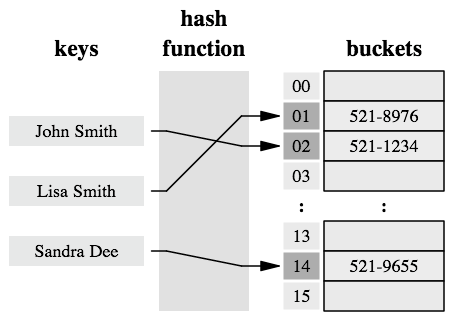
\includegraphics[angle=0,width=0.5\textwidth]{Fig_1}
\end{center}
\caption{Figura d'esempio}
\end{figure}


\section{La funzione di hash}

Nel caso in cui l'universo delle chiavi {\em U}  (l'insieme di tutte le chiavi possibili), sia ragionevolmente piccolo, \`e possibile utilizzare {\em tavole a indirizzamento diretto} (di dimensione $|U|$) per cui alla chiave {\em k} corrisponde l'indice {\em k}. Tuttavia se l'universo delle chiavi \`e esteso, e l'insieme {\em K} delle chiavi effettivamente memorizzate \`e molto pi\`u piccolo rispetto a {\em U}, allocare una tavola di dimensione $|U|$ risulta inefficiente e talvolta persino impossibile: la funzione di hash riduce l'intervallo degli indici dell'array da gestire.
\\

%credo che questo esempio permetta di capire velocemente come funziona l'uso della funzione di hash, i vantaggi e il problema delle collisioni. L'esempio � tratto da http://www.pspc.unige.it/~strutturesw1/SSW1_0506/Tabelle_hash.pdf

{\em Esempio:

Si supponga di dover registrare informazioni associate a 100 studenti, ognuno con un proprio numero di matricola compreso tra $0$ e $99$. In questo caso risulta naturale memorizzare i dati in un array di 100 elementi, con relativi costi delle operazioni sull'array  limitati a $\Theta(1)$.

Se l'intervallo del numero di matricola fosse pi\`u ampio, per esempio $[0,99999]$, non sarebbe conveniente adottare un array di 100000 elementi, di cui solo 100 necessari. In questo caso \`e possibile adottare un array di 100 elementi e una funzione hash che trasformi il numero di matricola in un indice dell'array. La funzione hash pi\`u semplice \`e la seguente: }
\\

$h(k)=k \  $mod$ \ 100$
\\

{\em
In questo modo la chiave viene divisa per la dimensione della tabella e il resto della divisione  \`e usato come indice dell'array. Per esempio, alla matricola 19803 viene associato l'indice 3.

\begin{figure}[h]
\begin{center}
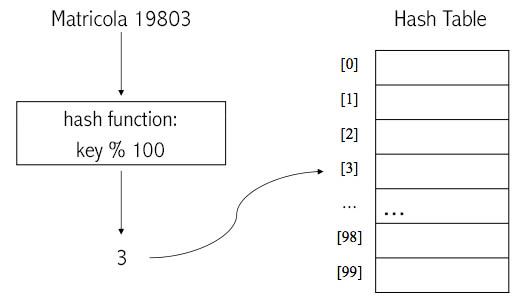
\includegraphics[angle=0,width=0.6\textwidth]{Esempio1}
\end{center}
\caption{Esempio di hash function}
\end{figure}

E' importante notare che in questo modo si perde l'ordine secondo il valore della chiave (lo studente 18865 dovrebbe precedere lo studente 19854). Inoltre \`e possibile che a due matricole venga associato lo stesso indirizzo (per esempio ci\`o accade con le matricole 19865 e 19765): questo evento viene chiamato collisione.
}
\\

La funzione di hash ha il compito di trasformare un certo dato {\em k}, chiave di un elemento, in un intero compreso tra 0 ed $m-1$ utilizzato come indice di un array di dimensione $m$.
In altri termini, se {\em U} \`e l'universo delle chiavi, la funzione hash {\em h} associa ad una chiave {\em k} il suo {\em valore hash h(k)}. 
\\

$h : U \rightarrow \{0,1,...,m-1\}$
\\

La funzione hash deve avere le seguenti caratteristiche:
\begin{itemize}
\item Deve essere semplice per non appesantire il programma;
\item Deve associare a due chiavi uguali lo stesso valore di hash;
\item Deve essere deterministica: dato un input $k$, l'output $h(k)$ deve essere sempre lo stesso.
\end{itemize}

Il problema che si presenta adottando la funzione di hash \`e quello delle {\bf collisioni}: due chiavi possono essere associate alla stessa posizione nell'array.

\section{Collisioni}

Il caso in cui la funzione hash applicata a due chiavi diverse genera un medesimo indirizzo viene chiamato collisione.
Le collisioni rappresentano un problema da arginare per quanto possibile scegliendo un'opportuna funzione hash. Eliminare completamente le collisioni \`e impossibile: se, come precedentemente riportato, $m < |U|$, devono esistere {\em almeno} due chiavi in $U$ a cui corrisponde lo stesso valore di hash.

Un primo approccio al problema consiste nell'adottare una funzione di hash che limiti per quanto possibile la frequenza delle collisioni, per esempio mediante una mappatura che sembri "casuale" (naturalmente la funzione deve essere deterministica).

In secondo luogo \`e necessario adottare determinate procedure per gestire le collisioni quando queste si verificano.

\subsection{Gestione delle collisioni mediante concatenamento}
Con il {\bf concatenamento}, tutti gli elementi che sono associati alla stessa cella vengono inseriti in una lista concatenata. Ogni cella della tabella di hash contiene dunque il puntatore alla testa di una lista di tutti gli elementi che corrispondono a quella determinata cella (la lista pu\`o essere vuota, avere un elemento o pi\`u elementi). L'inserimento di un elemento nel caso peggiore ha un costo $O(1)$, in quanto l'elemento viene inserito alla testa della lista, e la lista non viene visitata.

Per quanto riguarda le prestazioni in termini di ricerca di un elemento, il tempo di esecuzione nel caso peggiore \`e proporzionale alla lunghezza della lista. \`E possibile che tutti gli elementi vengano associati allo stesso indice: in questo caso l'intera tabella di hash degenera in una lista, le cui prestazioni sono basse; infatti, il costo di ricerca per una lista concatenata \`e lineare $O(n)$, dove $n$ corrisponde al numero di elementi nella lista.

Per avere un'idea generica delle prestazioni di una tabella di hash con concatenamento, viene definito un {\bf fattore di carico} $\alpha$, uguale al rapporto tra il numero $n$ di elementi memorizzati e le dimensioni della tabella di hash $m$. In una prima approssimazione \`e consigliabile che il fattore di carico $\alpha$  non superi i valori 4 o 5, per evitare la formazione di liste eccessivamente lunghe. Ovviamente questa considerazione non esclude la necessit\`a di una funzione hash che distribuisca in modo efficace gli elementi nell'array.
\\

\begin{figure}[h]
\begin{center}
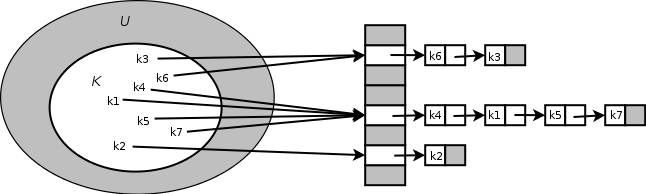
\includegraphics[angle=0,width=0.9\textwidth]{Chaining}
\end{center}
\caption{Rappresentazione della procedura di concatenamento}
\end{figure}

\subsection{Gestione delle collisioni mediante indirizzamento aperto}
Adottando l'{\bf indirizzamento aperto}, tutti gli elementi sono memorizzati nella tavola hash e non sono presenti liste esterne alla tabella o puntatori. 

Nel caso pi\`u semplice di indirizzamento aperto a  {\bf ispezione lineare}, se un elemento viene associato ad una cella gi\`a occupata, si ispezionano le celle successive finch\'e non ne viene trovata una vuota in cui inserire l'elemento. Una seconda funzione di hash $h'(k,i)$ viene chiamata in caso di collisione:
\\

$h'(k,i) = (h(k)+i) \ $mod$  \ m$
\\

La variabile $i$, inizialmente $i=1$, viene incrementata ogni volta che si procede con l'ispezione della cella successiva. Il valore di $i$ non pu\`o superare le dimensioni della tabella di hash. 

Quando \`e necessario eseguire la ricerca di un elemento, si usa il valore di hash per trovare l'indice dell'array da ispezionare; se l'elemento nella cella non corrisponde a quello desiderato si procede ispezionando le posizioni dell'array con indici successivi fino a quando l'elemento non viene trovato o fino a quando non viene raggiunta una cella vuota. In quest'ultimo caso l'elemento richiesto non \`e presente nella lista. 
\\

L'indirizzamento aperto ad ispezione lineare presenta un problema noto come {\bf addensamento primario}: si formano lunghe file di celle consecutive occupate che aumentano il tempo medio di ricerca. 

Per ridurre l'effetto di addensamento si pu\`o considerare un'{\bf ispezione quadratica}, la cui funzione hash chiamata in caso di collisione \`e la seguente:
\\

$h'(k,i) = (h(k) + c_1i + c_2i^2)$ mod $m$
\\

Le costanti ausiliarie $c_1$ e $c_2$ devono essere diverse da zero.
\\
%Si pu� inserire un esempio di ispezione quadratica o di doppio hashing per facilitarne la comprensione del funzionamento

Uno dei migliori metodi disponibili per l'indirizzamento aperto \`e quello del {\bf doppio hashing} in cui $h'(k,i)$ include due diverse funzioni $h_1(k)$ e $h_2(k)$, opportunamente configurate:
\\

$h'(k,i) = (h_1(k) + ih_2(k))$ mod $m$;
\\

Diversamente dai casi di ispezione lineare e quadratica, con il doppio hashing la sequenza di ispezione dipende in due modi dalla chiave $k$, perch\'e possono variare sia la posizione iniziale di ispezione sia la distanza tra due posizioni successive di ispezione.
\\

Quando un elemento deve essere cancellato dalla tabella di hash a indirizzamento aperto,  \`e necessario marcare la cella come DELETED: ripristinare la cella come vuota potrebbe infatti impedire all'algoritmo di ricerca di trovare gli elementi per il cui inserimento sia stata esaminata la cella in questione trovandola gi\`a occupata.

Nel caso di indirizzamento aperto il fattore di carico $\alpha$ non pu\`o essere maggiore di 1, in quanto il numero di elementi che si possono memorizzare \`e limitato dalla dimensione della tabella di hash. Eccessive collisioni, con conseguente allungamento dei tempi di ispezione, possono compromettere la prestazione della struttura dati; in prima approssimazione \`e dunque consigliabile mantenere $\alpha < 0,75$.




\end{document}  
\`e